\section{Konfiguration und Bauen des Systems}
\label{cha:ver:sec:Konfiguration_und bauen_system}

In diesem Abschnitt werden vor allem die Werkzeuge erläutert, die zur Erstellung einer angepassten Linux-Distribution benötigt werden, sowie die Methode, mit der eine solche Distribution erstellt wird. Dabei wird ein Überblick über das Yocto-Projekt als Grundlage für die PetaLinux-Werkzeuge gegeben. Der Prozess der Erstellung einer Linux-Distribution mit den PetaLinux-Tools wird beschrieben. Darüber hinaus wird der Prozess der Konfiguration und Erstellung des Kernels und des Root-Dateisystems für den Zynq UltraScale+ MPSoC im Detail erklärt. \\
Um den PetaLinux-Build Prozess zu verstehen, ist es wichtig, bestimmte Schlüsselkonzepte im Zusammenhang mit dem Yocto-Projekt zu verstehen, darum wird in dem nächsten Abschnitt erst das Yocto-Projekt vorgestellt. 

\subsection{Das Yocto Projekt}

Die Arbeit mit dem Yocto-Projekt ist die Basis für die Erstellung einer Linux-Distribution mit den PetaLinux-Tools. Die PetaLinux-Tools nutzen den Build-Prozess des Yocto-Projekts zur Erstellung der Linux-Distribution und verbergen damit die Komplexität, die mit der direkten Verwendung des Yocto-Projekts einhergeht. Sie bieten eine einfach zu bedienende Kommandozeilenschnittstelle, die es Entwicklern erleichtert, das Betriebssystem zu erstellen. \\
Das Yocto-Projekt jedoch  ist ein Open-Source-Projekt, das auch Entwicklern hilft, angepasste Linux-Distributionen für ihre eingebetteten Systeme zu erstellen, die verschiedene Prozessorarchitekturen unterstützen. Um die Distribution zu erstellen, verfügt das Projekt über eine Sammlung von Werkzeugen und Mechanismen zur Erstellung von angepassten Komponenten wie FSBL, U-Boot, Device-Tree und Kernel-Image zum Booten von Linux auf Embedded-Systemen.\\
Das Yocto-Projekt verwendet ein Schichtenmodell(Layer Model), das den Benutzern die Flexibilität bietet, schichtspezifische Änderungen vorzunehmen. 

\subsubsection{Yocto Layer}

Yocto-Layer oder Meta-Daten-Layer sind Repositories von Konfigurations- und Build-Skripten zusammen mit Build-Spezifikationen (BitBake-Rezepten), die dem Yocto-Build-System (OpenEmbedded Build System) mitteilen, wie eine angepasste Linux-Distribution zu bauen ist. Sie können hardwarespezifisch sein, oder so flexibel sein, dass sie auch für andere Architekturen angepasst werden können
Je nachdem, wie komplex der Entwickler eine bestimmte Schicht gestalten möchte, können Layer verwendet werden, um bestimmte Build-Aufgaben zu trennen oder zu kombinieren. Die Erhöhung der Build-Aufgaben, die mit  bestimmten Layers verbunden sind, erhöht die Komplexität des Projekts und erschwert den Entwicklern die Anpassung, Wartung und Wiederverwendung von diesen Layers. Abbildung ~\ref{fig:bblayers} zeigt die Ausgabe einer typische bblayers.conf Datei.

\begin{figure}[H]
	\begin{center}		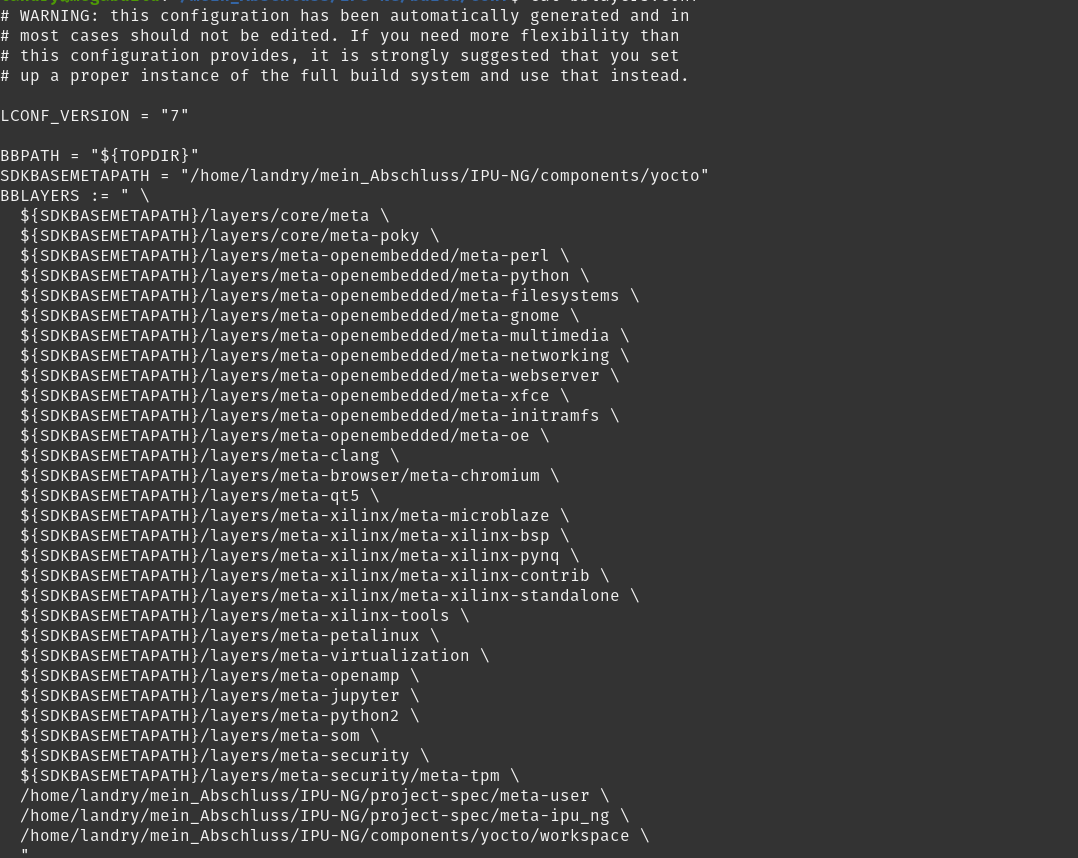
\includegraphics[width=1\textwidth]{./images/bblayer_datei.jpg}
	\end{center}
	\vspace{-5pt}
	\caption[Menuconfig Startbildschirm des PetaLinux-Projekts]{Menuconfig Startbildschirm des PetaLinux-Projekts} % Eckige Klammer (optional): Caption-Text in Abbildungsverzeichnis
	\label{fig:bblayers}
	\vspace{-5pt}
\end{figure}



\subsubsection{Poky}
Bei Poky handelt es sich um eine Referenzdistribution, die vom Yocto-Projekt verwendet wird, um eigene Linux-Distributionen zu erstellen. Sie besteht aus dem OpenEmbedded Build-System und den Metadaten, die dem Build-System helfen, eine minimale Linux-Distribution zu erstellen. Die minimale Linux-Distribution, die mit Poky erstellt wurde, wird mit weiteren Meta-Layern wie meta-xilinx und meta-petalinux angepasst, um das Linux-Image für Xilinx-Prozessoren anzupassen. Bei den Metadaten handelt es sich im Wesentlichen um Konfigurationsskripte und BitBake-Rezeptdateien.

\subsubsection{Bitbake Engine}

Wie in der Bitbake-Dokumentation beschrieben, handelt es sich bei Bitbake um eine Build-Engine, die vom Yocto-Projekt zur Erstellung von Linux-Distributionen verwendet wird. Genau wie der Linux-Kernel ist sie in der Lage, die in den OpenEmbedded-Build-Skripten beschriebenen Aufgaben parallel auszuführen, zu verwalten und zu koordinieren. Darüber hinaus stellt die Bitbake-Engine sicher, dass jede Aufgabe die erforderlichen Ressourcen für die Ausführung hat, indem sie BitBake-Rezepte verwendet. Dies sind Dateien die die Endung ".bb"\ tragen.

\subsubsection{Bitbake Recipes(Bitbake Rezept)}
In diesem Abschnitt möchte ich die Bitbake-Rezepte beschreiben, da im nächsten Paragraphen ein paar Rezepte geschrieben werden. 
Rezepte sind die von BitBake verwendeten grundlegenden Metadaten-Dateien, die mit der Dateinamenerweiterung .bb gekennzeichnet sind. Das Ziel wäre es, ein oder mehrere Ausgabepakete mit diesen Rezepten zu erhalten, die dann in das rootfs integriert werden können. folgenden wichtige Informationen sollten Datei vorhanden sein: 
\begin{itemize}
	\item Wichtige Informationen über das Rezept wie z. B. die Version, den Autor, die Homepage und die Lizenz
	\item Build- und Laufzeit-Abhängigkeiten
	\item Pfad zur Quellcode und wie man ihn abruft
	\item Mögliche Patches für den Quellcode und wie sie angewendet werden können
	\item Konfiguration und Kompilierung des Quellcodes
	\item wie und wo die generierten Build-Produkte zu installieren sind
\end{itemize}
Die wesentlichen Aufgaben, die vom Build-System beim Parsen eines Rezepts in der angegebenen Reihenfolge ausgeführt werden, sind die folgenden[\cite{YoctoProj}]

\begin{description}
	\item[do_fetch:] Diese Funktion lädt den Quellcode von einer angegebene Pfad Variable SRC_URI herunter. 
	\item[do_unpack:] entpackt die heruntergeladenen Daten
	\item[do_patch:] fügt Patches auf den Quellcode ein
	\item[do_configure:] konfiguriert den gesamten Quellcodebaum.
	\item[do_compile:] kompiliert den vorbereiteten Quellcode
	\item[do_stage:] legt die Kompilierungsergebnisse im Verfügungsbereich ab.
	\item[do_install:] sorgt dann für die Einrichtung des Pakets im Paketbereich.
	\item[do_package:] erstellt ein Paket, das die gewünschte Ausgabe enthält.
\end{description} 

Die resultierende Pakete oder Module werden dann im Rootfs eingefügt
\subsection{Konfigurieren des PetaLinux-Projekts}
Wie im Abschnitt  ~\ref{sec:Petalinux_Toolflow:petalinux:kommando} gut beschrieben, wird das Petalinux Kommando \textbf{petalinux-config} zur konfigurieren des Projekts verwendet. Bei der Konfiguration des Projekts ist es möglich die Board-Support-Pakete für ein Design in der Vivado Design-Suite zu erstellen, um einen Pfad zur Hardwar-Design-Datei während der Konfigurationsphase anzugeben, verwendet man die Option \textbf{--get-hw-description} wie im ~\ref{sec:Petalinux_Toolflow:petalinux:kommando} erklärt. \\
Mit diesem Befehl kann PetaLinux die Linux-Distribution entsprechend der bereitgestellten Hardwarebeschreibungsdatei (HDF) konfigurieren. Die Übergabe des Pfades zum BSP hilft bei der Generierung der Konfiguration für die Erstellung des korrekten Device-tree, FSBL, U-Boot und der Kernel-Treiber, die zum Booten von Linux auf der Xilinx-Plattform erforderlich sind.

\begin{figure}[H]
	\begin{center}		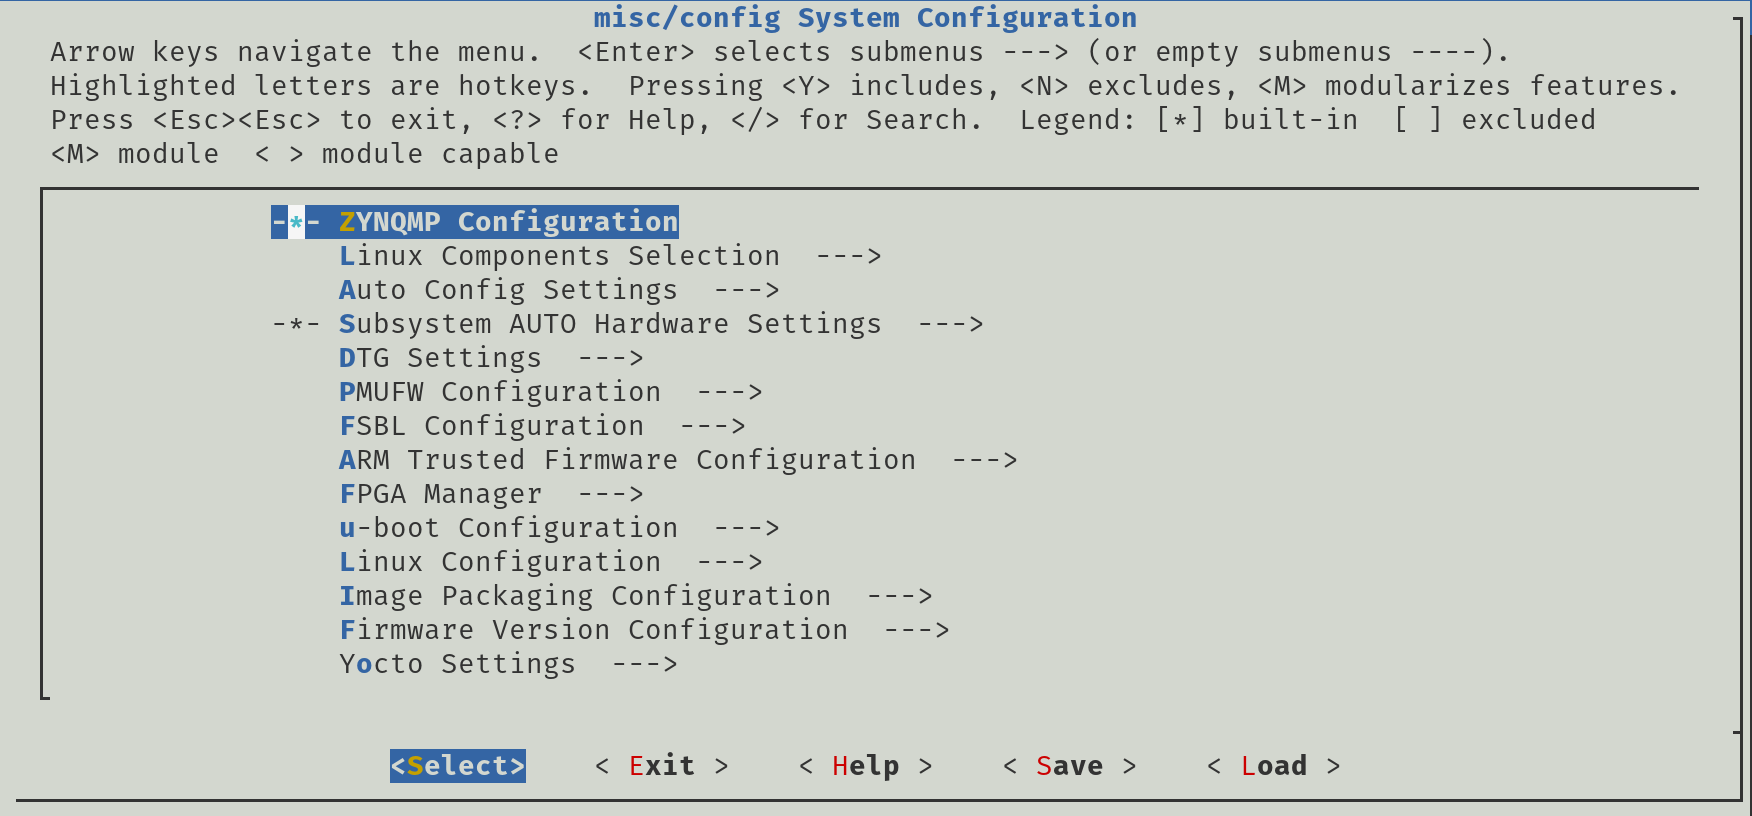
\includegraphics[width=1\textwidth]{./images/petalinux_config.jpg}
	\end{center}
	\vspace{-5pt}
	\caption[Menuconfig Startbildschirm des PetaLinux-Projekts]{Menuconfig Startbildschirm des PetaLinux-Projekts} % Eckige Klammer (optional): Caption-Text in Abbildungsverzeichnis
	\label{fig:menuconfig}
	\vspace{-5pt}
\end{figure}

Die Abbildung ~\ref{fig:menuconfig} zeigt der Menuconfig Startbildschirm, der erscheint, nachdem der Befehl \textbf{petalinux-config} die nach dem Befehl \textbf{petalinux-create} erzeugten Kconfig-Dateien analysiert hat. Diese Menuconfig ist eigentlich ausreichend, um das gesamte Projekt zu konfigurieren, aber man kann jedoch auch individuelle Konfigurationen für Boot-Komponenten mit einer ähnlichen Menuconfig-Schnittstelle vornehmen. Diese Individuelle Komponenten Konfigurationen sind nämlich wichtig wenn man  komplexe Konfigurationen vornehmen soll. So gibt es eine Menuconfig für den Kernel, das U-boot, das Rootfs ...\\
Damit unser MCP251xfd CAN-Controller erkannt und in Betrieb genommen werden kann, sollte man z.B. das Kernel-Menüocnfig verwenden, um den Treiber zu integrieren. Absichtlich wurde Petalinux 2021 verwendet, da für den Chip ein Treiber vorhanden ist. 

\begin{figure}[H]
	\begin{center}		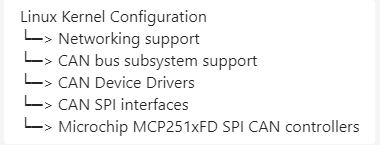
\includegraphics[width=0.7\textwidth]{./images/mcp_driver_pfard.jpg}
	\end{center}
	\vspace{-5pt}
	\caption[Pfard zur mcp251xfd Treiber]{Pfard zur mcp251xfd Treiber} % Eckige Klammer (optional): Caption-Text in Abbildungsverzeichnis
	\label{fig:mcp:treiber:pfard}
	\vspace{-5pt}
\end{figure}

Der oben gezeigte Pfad führt uns zum Kernel-Fenster, wo man den Treiber für den MCP251xFD aktivieren oder deaktivieren kann. Die Abbildung ~\ref{fig:mcp:treiber} zeigt alle CAN-Controller mit SPI-Schnittstelle, die uns der Kernel 5.10 bietet. Hier können sie auch als Modul aktiviert werden, so dass der Treiber nach dem Bootvorgang geladen oder entladen werden kann. Dies wurde in dieser Arbeit genutzt, um zu überprüfen, ob der Treiber den Mikrochip korrekt initialisiert hat.

\begin{figure}[H]
	\begin{center}		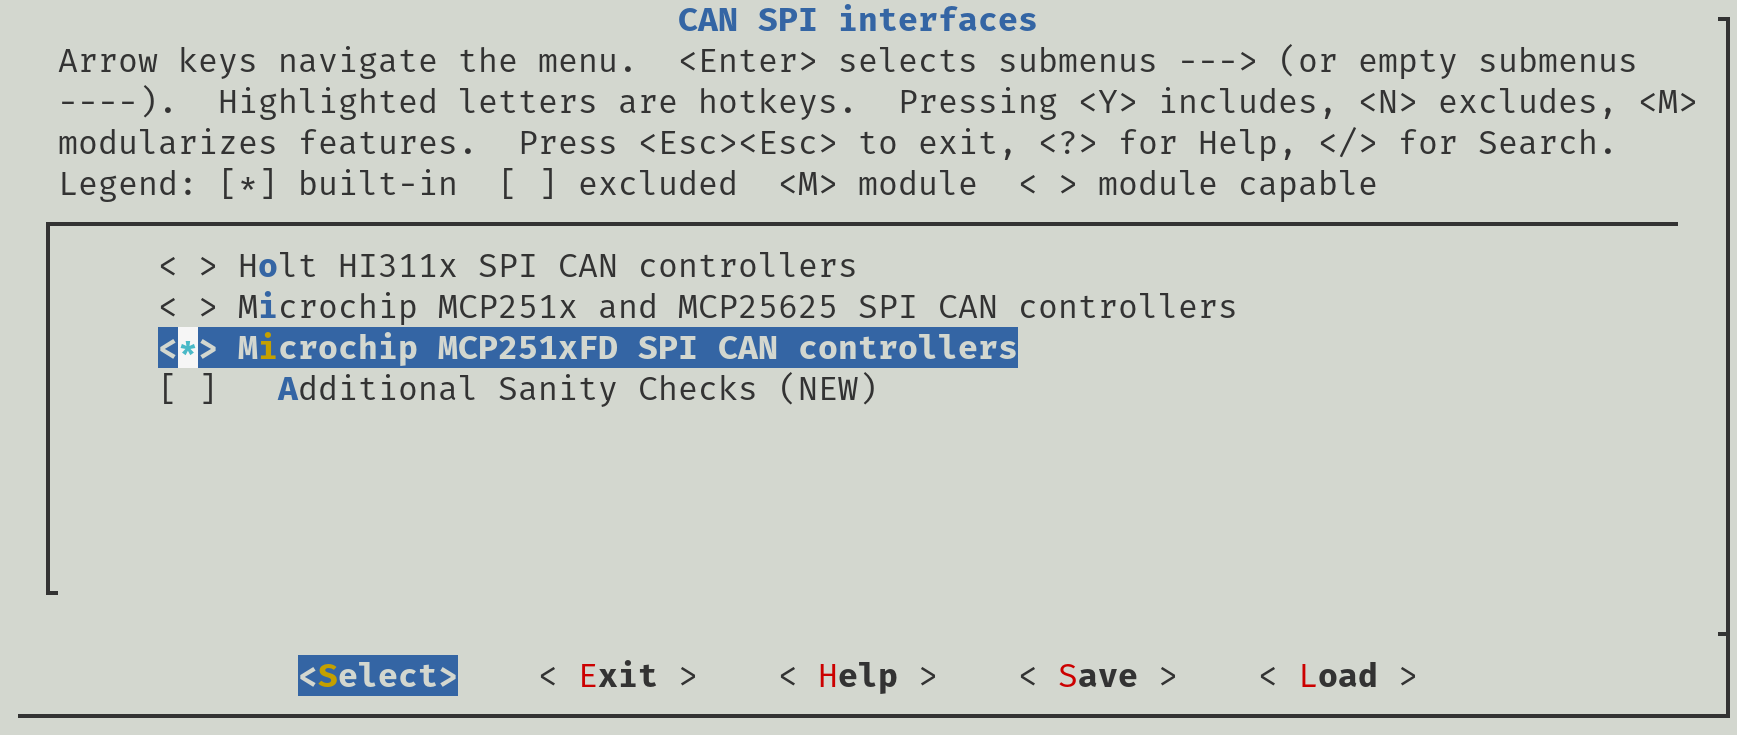
\includegraphics[width=1\textwidth]{./images/mcp_treiber.jpg}
	\end{center}
	\vspace{-5pt}
	\caption[Konfig Fenster mcp251xfd Treiber]{Konfig Fenster mcp251xfd Treiber} % Eckige Klammer (optional): Caption-Text in Abbildungsverzeichnis
	\label{fig:mcp:treiber}
	\vspace{-5pt}
\end{figure}

\subsection{Device-Tree Eintrag für den MCP251XFD CAN-Controller }
\begin{figure}[H]
	\begin{center}		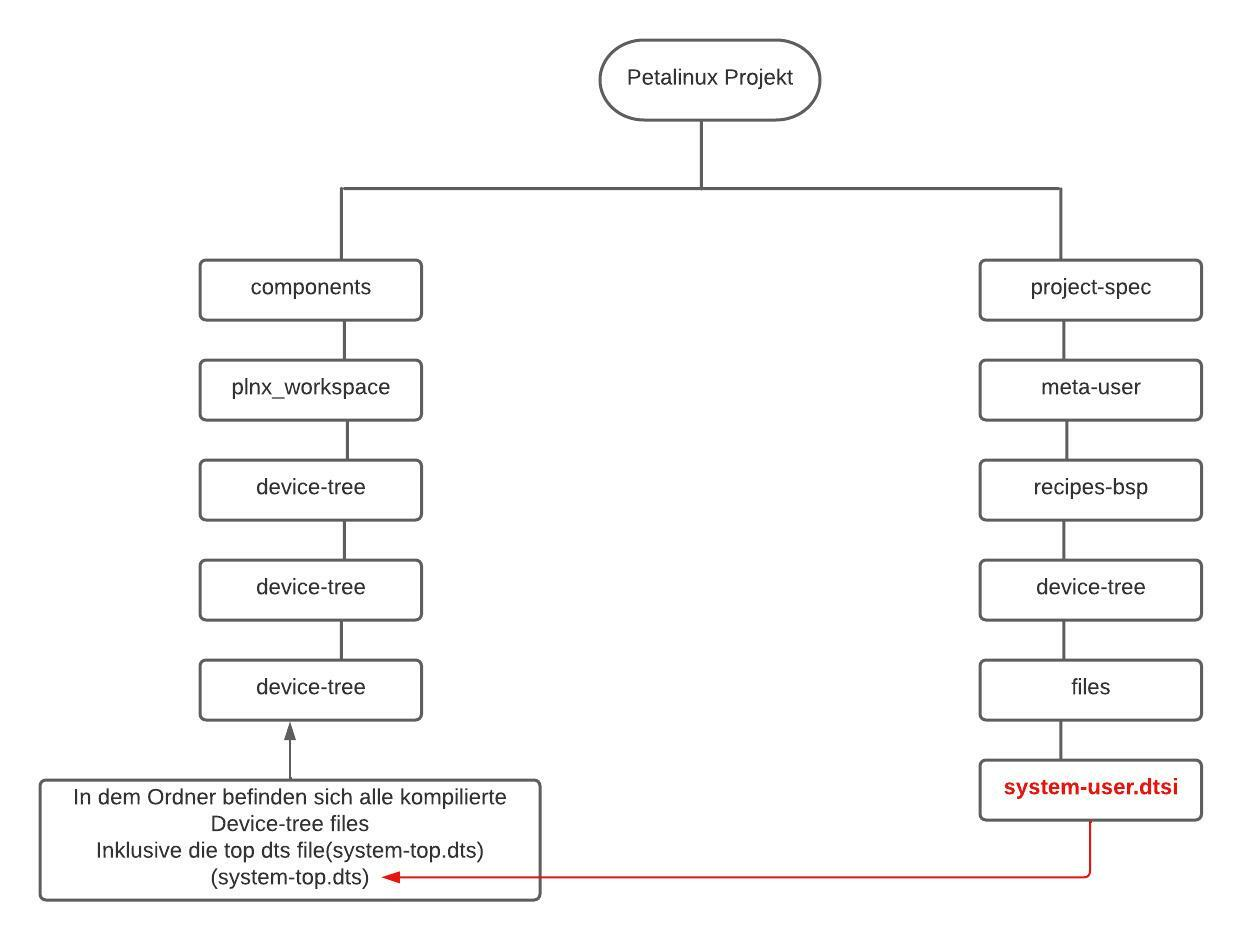
\includegraphics[width=1\textwidth]{./images/device-tree-diagram.jpg}
	\end{center}
	\vspace{-5pt}
	\caption[Device-tree Projekt Struktur]{Device-tree Projekt Struktur} % Eckige Klammer (optional): Caption-Text in Abbildungsverzeichnis
	\label{fig:deviceTree:struktur}
	\vspace{-5pt}
\end{figure}

Damit unser Mikrochip nach dem Bootvorgang in Betrieb genommen werden kann, müssen dem Kernel Informationen (wie z.B. der Name des Hardwaretreibers, die Taktfrequenz oder der Interrupt-Pin...) übergeben werden, damit die Hardware während des Bootvorgangs initialisiert wird. Daher wird in Petalinux empfohlen, die Datei \textbf{system-user.dtsi} zum Hinzufügen, Löschen oder Ändern eines Gerätebaumknotens zu verwenden. Diese Datei befindet sich in \textbf{<project>/project spec/meta-user/recipes-bsp/device-tree/files/}. Sie wird an das Ende der Datei system-top.dts gestellt wie im Listing ~\ref{lst:device:tree:top} dargestellt, so dass sie eine höhere Priorität erhält, und wird somit zuerst kompiliert.

%\newpage
%or \small or \footnotesize etc.
\begin{lstlisting}[backgroundcolor = \color{lightgray},basicstyle=\scriptsize\ttfamily,caption={Inhalt der system-top.dts Datei},label=lst:device:tree:top,language=bash,framexleftmargin = 2em]
/dts-v1/;
#include "zynqmp.dtsi"
#include "zynqmp-clk-ccf.dtsi"
#include "zcu106-reva.dtsi"
#include "pcw.dtsi"
/ {
	chosen {
		bootargs = "earlycon";
		stdout-path = "serial0:115200n8";
	};
	aliases {
		ethernet0 = &gem3;
		i2c0 = &i2c0;
		i2c1 = &i2c1;
		serial0 = &uart0;
		serial1 = &uart1;
		spi0 = &qspi;
		spi1 = &spi0;
	};
	memory {
		device_type = "memory";
		reg = <0x0 0x0 0x0 0x7ff00000>, <0x00000008 0x00000000 0x0 0x80000000>;
	};
};
#include "system-user.dtsi"	
\end{lstlisting}

Das Petalinux-Projekt wurde mit einer von Vivado exportierten Hardwarebeschreibungsdatei (HDF-Datei) konfiguriert, in der bestimmte Vorkonfigurationen bereits vorgenommen wurden. Beispielsweise die Konfiguration der Pins, des gpio-Controllers, des SPI-Controllers usw. 

\begin{figure}[H]
	\begin{center}		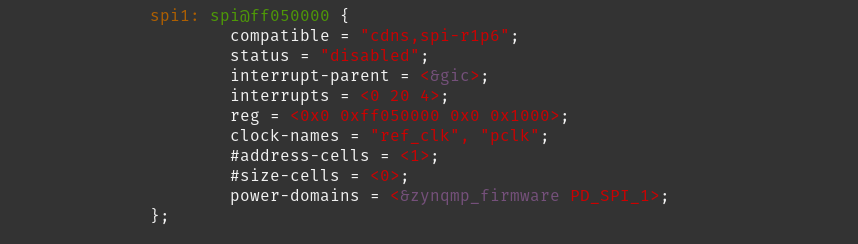
\includegraphics[width=1\textwidth]{./images/xilinx_spi_controller.jpg}
	\end{center}
	\vspace{-5pt}
	\caption[Xilinx SPI-Controller]{Xilinx SPI-Controller} % Eckige Klammer (optional): Caption-Text in Abbildungsverzeichnis
	\label{fig:deviceTree:spi:controller}
	\vspace{-5pt}
\end{figure}

Der Code, der in Abbildung ~\ref{fig:deviceTree:spi:controller} zu sehen ist. beschreibt den im Vivado implementierten Xilinx-SPI-Controller, an den unserer CAN-Controller angeschlossen werden soll. im \textbf{reg} ist die Basisadresse und der Adressbereich, in dem der SPI-Controller betrieben wird. \\
Der Code, der in den aktuellen Device-tree für den CAN-Controller eingefügt werden muss, ist der unten stehende.
\begin{lstlisting}[backgroundcolor = \color{lightgray},basicstyle=\scriptsize\ttfamily,caption={Device-tree Eintrag für den mcp251xfd CAN-Controller},label=lst:device:tree:mcp,language=bash,framexleftmargin = 2em]
	
	/include/ "system-conf.dtsi"
	/ {
		can0_osc: can0_osc {
			compatible = "fixed-clock";
			#clock-cells = <0>;
			clock-frequency = <20000000>;
		};
	};
	
	&spi0 {
		#address-cells = <1>;
		#size-cells = <0>;
		can@0 {
			compatible = "microchip,mcp251xfd";
			reg = <0>;
			clocks = <&can0_osc>;
			pinctrl-names = "default";
			//pinctrl-0 = <&can0_pins>;
			interrupts-extended = <&gpio 78 8>;
			spi-max-frequency = <8333333>;
			microchip,rx-int-gpios = <&gpio 79 1>;
		};
	};
\end{lstlisting}

wichtige Information dazu wurde in den folgende Tabelle zusammengefasst. 

\begin{tabular}{lp{11cm}}
	\toprule
	\textbf{Funktion} &\textbf{Beschreibung}\\
	\midrule
	\textit{compatible} & wird verwendet, um zu entscheiden, wie das Gerät ausgeführt werden soll und das Gerät mit dem Treiber zu verbinden. Er enthält eine Zeichenkette in der Form <Hersteller>,<Modell>. In unseren Fall handelt es sich um ein microchip herstellte mcp251xfd.\\
	\textit{reg = <0>} & dem CAN-Controller wird eine eindeutige ID zugewiesen, der hat  also keine Adresse Bereich. \\
	\textit{clocks} & Der interne Taktgenerator im Controller wird hier beschrieben. Der kann 40, 20 oder 4 MHz generieren. Hier wurde er aber auf 20 MHz eingestellt.\\
	\textit{interrupts-extended} & Hier werden die vom Gerät erzeugten Interrupts aufgelistet. Es wird auch spezifiziert an welchem GPIO-Pin diese Interrupts empfangen werden.\\
	\textit{spi-max-frequency} & steht für die maximale SPI-Taktfrequenz des Geräts. Diese wurde auf 8,33 MHz gesetzt, da für eine gute Kommunikation mit dem SPI-Master die SPI-Taktfrequenz die Hälfte oder weniger des Takts betragen sollte. \\
	\bottomrule
\end{tabular}

\subsection{Rezepte zur Kompilierung der Software Modulen}
Für die Erstellung von Rezepte wurde im Rahmen dieser Arbeit das Petalinux-devtool verwendet. Das ist ein Werkzeug, welches das Yocto devtool benutzt, um Software zu bauen, zu testen und einzubinden. Mit dem "petalinux-devtool"\ Kommando kann man zum Beispiel:
\begin{itemize}
	\item neue Rezepte einfügen
	\item Quelle Code von existierenden Rezepte ändern
	\item Umbenennen einer Rezeptdatei im Arbeitsbereich
	\item Oder Rezepte kompilieren 
\end{itemize}

Um die neuen Änderungen vom Rest des Projekts zu isolieren, wurde eine neue Ebene erstellt, in die alle Änderungen geschrieben wurden.

	\subsubsection{Hinzufügen einer neue Layer zu BBLAYERS}
	Es wurde zuerst ein neue Ebene-Verzeichnis und dessen Konfigurationsverzeichnis erstellt. dafür wurde ein bestehende Layers konfigurationsdatei in das conf-Verzeichnis der meta-Layers kopiert und wie folgt geändert. Diese Datei enthält die Informationen, die von BitBake benötigt werden, um die Ebene und die darin enthaltenen Metadaten zu erkennen. Insbesondere enthält diese Datei die Variable \textbf{BBPATH}, die das Stammverzeichnis des Layers angibt, in dem BitBake alle Dateien finden soll, die von Rezepten geerbt werden. Außerdem gibt die Variable \textbf{BBFILES} die Pfade an, in denen BitBake erwartet, Rezepte zu finden. Abhängigkeiten zwischen Schichten müssen stattdessen durch die Variable \textbf{LAYERDEPENDS_*} ausgedrückt werden.

	\begin{lstlisting}[backgroundcolor = \color{lightgray},basicstyle=\scriptsize\ttfamily,caption={Hinzufügen neue Yocto-ebene},label=lst:ipu:ng:layer,language=bash,framexleftmargin = 2em]
		
	# We have a conf and classes directory, add to BBPATH
	BBPATH .= ":${LAYERDIR}"
	
	# We have recipes-* directories, add to BBFILES
	BBFILES += "${LAYERDIR}/recipes-*/*/*.bb \
	${LAYERDIR}/appends/*.bbappend"
	
	BBFILE_COLLECTIONS += "meta-ipu_ng"
	BBFILE_PATTERN_meta-ipu_ng = "^${LAYERDIR}/"
	BBFILE_PRIORITY_meta-ipu_ng = "8"
	LAYERSERIES_COMPAT_meta-ipu_ng = "gatesgarth"
	
	# Set a variable to get to the top of the meta-layer location
	HAB_BASE := '${LAYERDIR}'
	\end{lstlisting}

	Anschlissend sollte die neue Yocto-Layer mit Hilfe des Systemkonfiguration Menü zu der hauptkonfiguration Layers (BBLAYER) hinzugefügt werden. Die Datei enthält alle Verweise auf die Ebenen, die von BitBake während des Analyseprozesses der Rezepte gescannt werden.
	
	\begin{figure}[H]
		\begin{center}		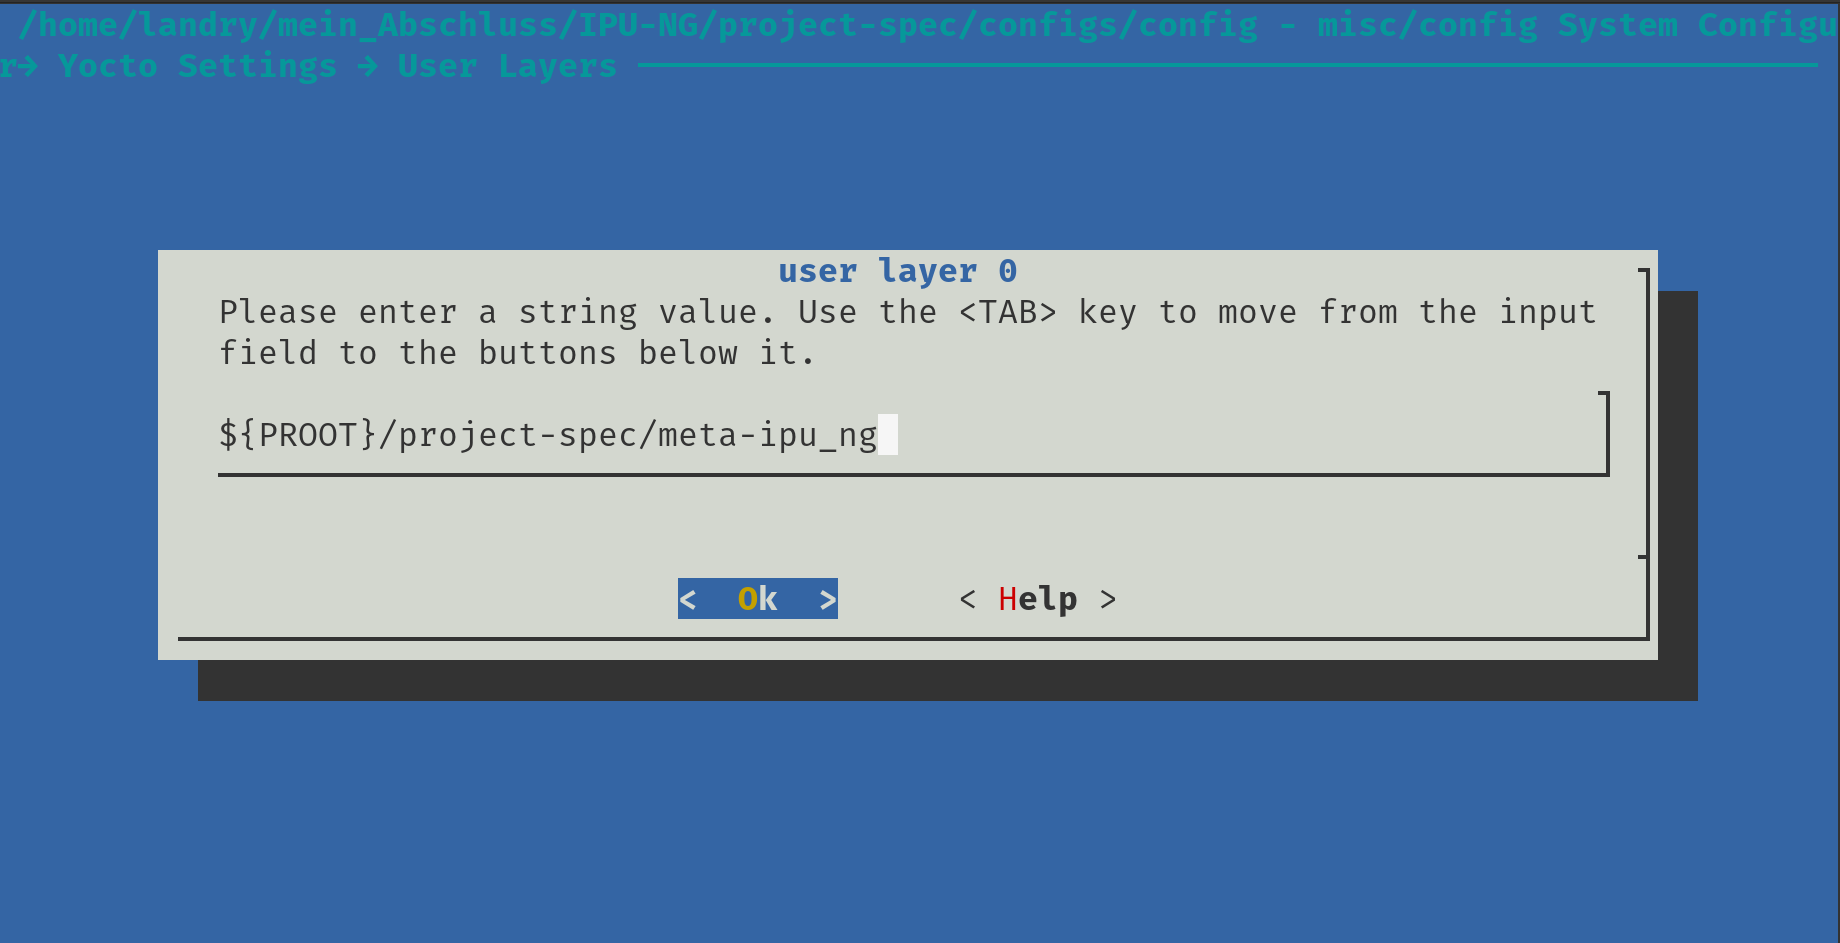
\includegraphics[width=0.8\textwidth]{./images/ip_ng_layer.jpg}
		\end{center}
		\vspace{-5pt}
		\caption[Neue Yocto-Ebene für IPU-NG Software Module]{Neue Yocto-Layer für IPU-NG Software Module} % Eckige Klammer (optional): Caption-Text in Abbildungsverzeichnis
		\label{fig:yocto_layer_ipu_ng}
		\vspace{-5pt}
	\end{figure}

Das Abbildung ~\ref{fig:bblayers} ist beispielsweise die Ausgabe der Datei \textbf{bblayers.conf} des Projekts. Am Ende können Sie sehen, dass die neue Layer am Ende der Datei eingefügt wird, nachdem das Projekt kompiliert wurde. 
	\subsubsection{Rezept zur Kompilierung der Software Modulen}
	Die folgen Variable wurden notwendig für die Erstellung der Rezepten. 
	\begin{description}
		\item[SUMMARY]: Diese Variable enthält einen String-Wert, den der Benutzer hilft zu wissen, worum es in dem Rezept geht.
		\item[LICENSE]: In dieser Variable ist die Art der Lizenz anzugeben, die man für das Rezept verwenden möchten. In unsere Fall ist es CLOSE, da man die in Firma entwickelte Software verwenden.
		\item[LIC_FILES_CHKSUM]: Diese Datei wird von dem OpenEmbedded-Build-System verwendet, um sicherzustellen, dass sich der Lizenztext nicht geändert hat. Diese Variable ist bei uns aber Leer, da wir die Liezens "CLOSE" verwenden.
		\item[PR]: Es geben wir das Revision Paket an. Der wurde in unsere Fall auf r0 gesetzt. 
		\item[PV]: definiert die Version des Rezepts
		\item[SRC_URI]: Hier wird der Pfad zum Quellcode der Software angegeben. In unserem Fall werden die Quellcodes vom Git-Server des Unternehmens abgerufen.
		\item[DEPENDS]: Hier werden Abhängigkeiten, die zur Kompilierungszeit gebraucht werden, angegeben.
		\item[S]: Hier gibt man das Quellverzeichnis an, in dem man die gesamte Erstellung durchführen kann.
	\end{description}
		
Das vom Yocto-Projekt unterstützte CMake Autotools wird im Rezept zum Konfigurieren, Kompilieren und Installieren der Software verwendet. Der Zweck dieser Werkzeuge ist es, die Arbeit des Programmierers zu erleichtern, indem mehrere Schritte des Erstellungsprozesses automatisiert werden. Nachfolgend sind die Rezepte zur Kompilierung der Software beschrieben.

\begin{lstlisting}[backgroundcolor = \color{lightgray},basicstyle=\scriptsize\ttfamily,caption={Rezept für das sw-main-app Modul},label=lst:sw_main_app:modul,language=bash,framexleftmargin = 2em]
	
	#
	# This file is the sw-main-app recipe.
	#
	
	SUMMARY = "sw-main-app applications"
	LICENSE = "CLOSED" 
	#LIC_FILES_CHKSUM = " "
	
	#PR = "r0"
	#PV = "1.0.5+git${SRCPV}"
	
	SRC_URI = "https://csp.edag.de/bitbucket/scm/ee21i00805/sw-main-app.git"
	PV = "1.0+git${SRCPV}"
	
	SRCREV = "${AUTOREV}"
	S = "${WORKDIR}/git"
	
	DEPENDS = "gstreamer1.0 gstreamer1.0-plugins-base glib-2.0 sw-system-module sw-system-logger"
	
	inherit cmake pkgconfig 
	
\end{lstlisting}

\begin{lstlisting}[backgroundcolor = \color{lightgray},basicstyle=\scriptsize\ttfamily,caption={Rezept für das sw-system-module Modul},label=lst:sw_system_module:modul,language=bash,framexleftmargin = 2em]
#
## This file is the sw-system-module recipe.
##
SUMMARY = "sw-system-module applications"
LICENSE = "CLOSED"
LIC_FILES_CHKSUM = ""

SRC_URI = "https://csp.edag.de/bitbucket/scm/ee21i00805/sw-system-module.git"

PV = "1.0+git${SRCPV}"
SRCREV = "${AUTOREV}"

S = "${WORKDIR}/git"
DEPENDS = "gstreamer1.0 gstreamer1.0-plugins-base glib-2.0"

inherit cmaken pkgconfig

\end{lstlisting}
\newpage
\begin{lstlisting}[backgroundcolor = \color{lightgray},basicstyle=\scriptsize\ttfamily,caption={Rezept für das sw-system-module Modul},label=lst:sw_system_logger:modul,language=bash,framexleftmargin = 2em]
#
#
## This file ist the sw-system-logger recipe
# 
SUMMARY = "sw-system-logger applications"                          
LICENSE = "CLOSED"
LIC_FILES_CHKSUM = ""

SRC_URI = "https://csp.edag.de/bitbucket/scm/ee21i00805/sw-system-logger.git"


PV = "1.0+git${SRCPV}"
SRCREV = "515609c99db34769320e54c5535cbfe58031839b"

S = "${WORKDIR}/git"
DEPENDS = "gstreamer1.0 gstreamer1.0-plugins-base glib-2.0 sw-system-module"

inherit cmake pkgconfig
\end{lstlisting}

Jede dieser Rezepte lassen sich mit dem folgenden Kommando kompilieren.
\begin{lstlisting}[language=bash]
	$ petalinux-devtool build <recipe_name>
\end{lstlisting}

Die resultierenden Softwarepakete wurden dann in rootfs aufgenommen, indem ein Eintrag in der Datei (\${PROOT}/project-spec/project-spec/meta-user/conf/user-rootfsconfig) erstellt wurde, wie in Listing ~\ref{lst:sw_paket:rootfs} dargestellt.

\begin{lstlisting}[backgroundcolor = \color{lightgray},basicstyle=\scriptsize\ttfamily,caption={Einbindung Software in Rootfs},label=lst:sw_paket:rootfs,language=bash,framexleftmargin = 2em]
#Note: Mention Each package in individual line
#These packages will get added into rootfs menu entry

CONFIG_gpio-demo
CONFIG_peekpok

CONFIG_sw-main-app
CONFIG_sw-system-module
CONFIG_sw-system-logger

CONFIG_gstreamer-vcu-examples
CONFIG_packagegroup-petalinux-v4lutils
CONFIG_packagegroup-petalinux-audio
	
\end{lstlisting}

Bevor die Software Pakete(sw-main-app, sw-system-logger, sw-system-module) schlißlich in Rootfs integriert werden können müssen sie noch in dem Rootfs Konfiguration Menü aktiviert werden.
\begin{figure}[H]
	\begin{center}		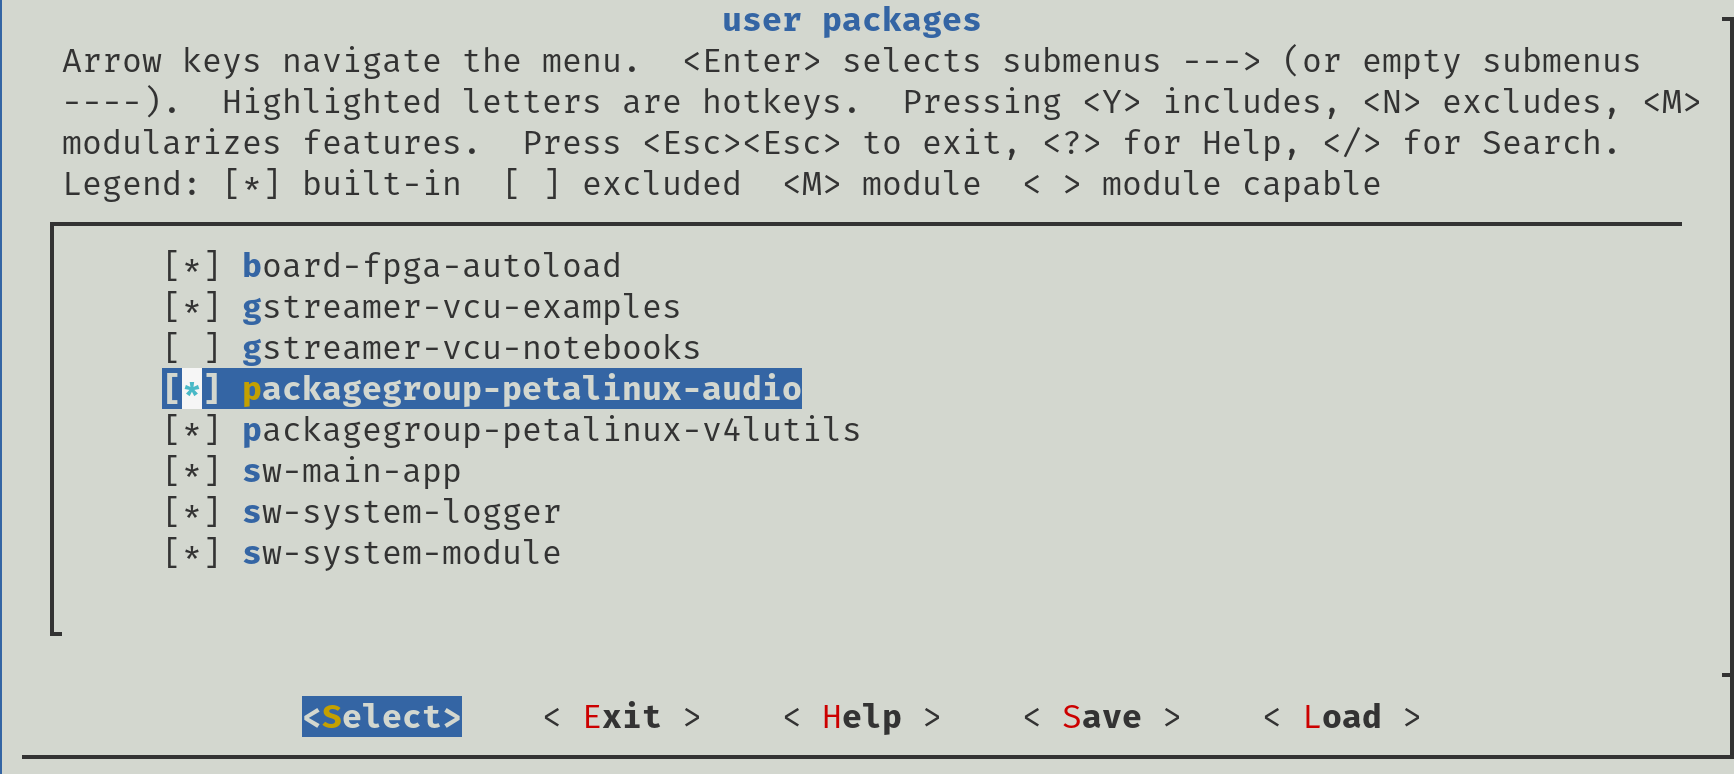
\includegraphics[width=1\textwidth]{./images/rootfs_config_sw.jpg}
	\end{center}
	\vspace{-5pt}
	\caption[Aktivierung Software Pakete in Rootfs]{Aktivierung Software Pakete in Rootfs} % Eckige Klammer (optional): Caption-Text in Abbildungsverzeichnis
	\label{fig:rootfs_config:sw}
	\vspace{-5pt}
\end{figure} 

\subsection{Bauen des Systems}
Nachdem alle Konfiguration gemacht wurden. könnte das Petalinux Projekt anschließend mit dem Kommando \textbf{petalinux-build} gebaut werden. Das petalinux-build Skript baut dann den Gerätebaum gemäß der HDF und der Treiberkonfiguration des Kernels auf, so dass der Treiber für den mcp251xfd CAN-Controller die Informationen über die Hardware am entsprechenden Knoten im Gerätebaum finden und die Hardware physisch lokalisieren kann.\\
Das \textbf{petalinux-build} erstellt auch das Root-Dateisystem für die PetaLinux-Distribution entsprechend der Kernelkonfiguration und der Metadaten in den erstellten Schicht.\\
Schließlich sollten nur noch die Boot Daten mit dem unten stehenden Befehl generiert werden.
\begin{lstlisting}[language=bash]
	$ petalinux-package --boot --fsbl images/linux/zynqmp_fsbl.elf --fpga ../bitstream/bd1_wrapper.bit --pmufw images/linux/pmufw.elf --u-boot --force
\end{lstlisting}

Sobald der Erstellungsprozess des PetaLinux-Projekts abgeschlossen ist, steht eine Reihe von bootfähigen Images zur Verfügung, die in der folgenden Tabelle beschrieben werden.\\


\begin{tabular}{lp{11cm}}
	\toprule
	\textbf{Erzeugte Datei} &\textbf{Beschreibung}\\
	\midrule
	\textbf{BOOT.BIN } & Diese Datei ist eine Sammlung von mehrere Images(Boot-Header, Partition-Header, und Image-Header).\\
	\textbf{system.bit} & Dies ist die Bitstream Datei. Sie enthält die Informationen, die für das FPGA notwendig sind, um die programmierbare Logik gemäß ihrer Konzeption zu konfigurieren. \\
	\textbf{pmufw.elf} & Dies ist die PMU-Firmware wie im Abschnitt ~\ref{cha:tech_grund:sec:Komponente_eines_Emb_Lin_Sys:sub:sec:pmu} beschrieben, läuft auf der PMU und wird nach dem Ausführen des PMU Boot-ROM geladen. \\
	\textbf{zynqmp_fsbl.elf} & Der FSBL ist der erste Bootloader, der auf der APU läuft. nähere Informationen findet man im Abschnitt ~\ref{cha:tech_grund:sec:Komponente_eines_Emb_Lin_Sys:sub:sec:fsbl} \\
	\textbf{u-boot.elf} & U-Boot ist die zweite Stufe des Bootloaders.Und wird im Paragraf ~\ref{cha:tech_grund:sec:Komponente_eines_Emb_Lin_Sys:sub:sec:fsbl} beschrieben \\
	\textbf{system.dtb} & Das ist die kompilierte Version des Gerätebaums(Device-tree). \\ 
	\textbf{Image} & Dies ist das generische binäre Linux-Kernel-Image. der zusammen mit dem DTB file können zur Ausführung des Linux-Betriebssystems verwendet werden.\\
	\textbf{image.ub} & Es handelt sich um ein FIT-Image (Flattened Image Tree), das aus dem Kernel-Image und dem Gerätebaum in einem einzigen Image besteht und von U-Boot verwendet werden kann.\\
	\textbf{bl31.elf } & Dad ist die ARM Trusted Firmware, die verwendet wird verwendet, um Übergänge zwischen der sicheren und der unsicheren Boot Modus zu behandeln. \\
	\bottomrule
\end{tabular}

Nach Abschluss alle diese Schritte haben wir nun alle notwendigen Elemente, um diese auf eine SD-Karte zu laden. In Dem nächsten Schritt wird die SD-Karte so formatiert werden, dass sie für das eingebettete Linux-Betriebssystem geeignet ist.
Hierfür sollten 2 Partitionen auf der SD-Karte erstellt und formatiert werden. So dass die erste die Boot-Partition und die zweite die Root-Partition ist. 

\begin{figure}[H]
	\begin{center}		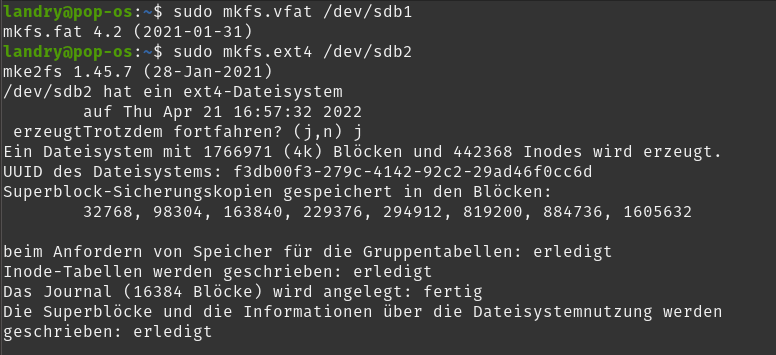
\includegraphics[width=0.8\textwidth]{./images/sd-karte_format.jpg}
	\end{center}
	\vspace{-5pt}
	\caption[Formatierung der SD-Karte Partitionen]{Formatierung der SD-Karte Partitionen} % Eckige Klammer (optional): Caption-Text in Abbildungsverzeichnis
	\label{fig:sd_karte:formatieerung}
	\vspace{-5pt}
\end{figure}

Nach diesem Schritt können die generierte Dateien auf die SD-Karte geschrieben werden. \\
Die Dateien BOOT.BIN boot.scr und image.ub sollten aus <plnx-proj-root>/pre built/linux/images/ in der Boot-Partition, die in FAT32-Format formatiert wurede, kopiert werden. der folgende Befehl wurde vom Petalinux Projekt angegeben.

\begin{lstlisting}[language=bash]
	$ sudo cp -v BOOT.BIN boot.scr image.iu /media/landry/0F4B-72BB
\end{lstlisting}

Um das Root-Dateisystem auf die Root-Partition zu schreiben, wurde den folgenden Befehl eingegeben.
\begin{lstlisting}[language=bash]
 	$ sudo tar xvf ./images/linux/rootfs.tar.gz -C /media/landry/f3db00f3-279c-4142-92c2-29ad46f0cc6d
\end{lstlisting}

\subsection{Booten des eingebetteten Linux-Images und Test des MCP251xfd CAN-Controller}
Damit ich die Möglichkeit habe, den Bootvorgang zu debuggen und eventuelle Fehlermeldungen herauszufinden, habe ich beschlossen, die Hardware-Plattform im JTAG-Modus zu booten. Der JTAG-Boot kommuniziert mit dem Xilinx ilinx System Debugger(XSDB), das wiederum mit dem hw_server über den TCP-Port 3121 kommuniziert. ein Tool command language (TCL) Script wird über das \textbf{petalinux-boot} Kommando ausgeführt, um die Zynqmp Plattform über JTAG zu starten. Das Skript sendet Befehle und Binärdateien über das Netzwerk an dem Remote-Hardware-Server, die die Boot Schritte repräsentieren.
der Terminal Emulator Programm Picocom wird hier verwendet, um die Bootmeldungen anzuzeigen. \\
Die folgenden schritte wurden durchgeführt, um Linux zu booten. 
\begin{itemize}
	\item Mit Hilfe einer JTAG Kabel, ist der JTAG Anschluss des Boards mit dem Hostrechner zu verbinden
	\item das gleiche gilt auch mit der serielle Schnittstelle 
	\item Der Modus-Schalter der Plattform sollte auf den JTAG-Modus umgestellt werden, indem die 4 Schalter auf \textbf{ON} geschaltet werden.
	\item Die Baudrate zur Kommunikation mit Picocom sollte eingestellt werden. 
	\begin{lstlisting}[language=bash]
		$ sudo picocom /dev/ttyUSB0 -b 115200
	\end{lstlisting}
	\item Erstellung einer Verbindung zu einem entfernten GDB-Server mit Hilfe des XSDBs
	\item Mit dem folgenden Befehl lässt sich Linux Booten.
	\begin{lstlisting}[language=bash]
	petalinux-boot --jtag --fpga --bitstream images/linux/system.bit --kernel
	\end{lstlisting}
\end{itemize}

Nachdem das Betriebssystem vollständig gebootet hat, kann man den Treiber mit den folgenden Befehlen entladen bzw. laden und überprüfen, ob der Treiber die Hardware korrekt initialisiert hat.  
\begin{lstlisting}[language=bash]
	$ rmmod mcp251xfd
	$ modprobe mcp251xfd
\end{lstlisting}
Abbildung ~\ref{fig:treiber:ladung} zeigt die Ausgabe des \textbf{modprobe} Kommandos aus. Da kann sehen dass die Hardware mit den richtigen Taktfrequenz initialisiert wurde. 
\begin{figure}[H]
	\begin{center}		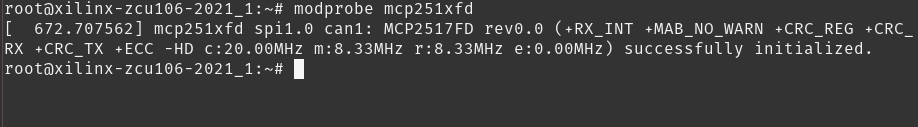
\includegraphics[width=1\textwidth]{./images/mcp_treiber_initialisietung.jpg}
	\end{center}
	\vspace{-5pt}
	\caption[Laden des mcp251xfd Treibers]{Laden des mcp251xfd Treibers} % Eckige Klammer (optional): Caption-Text in Abbildungsverzeichnis
	\label{fig:treiber:ladung}
	\vspace{-5pt}
\end{figure}

Ab jetzt kann die CAN Schnittstelle konfiguriert und getestet werden. Die wichtigsten Konfigurationen sind hier die Bit- und Datenrate, die über den IP-Kommando eingestellt werden können. Außerdem muss die Schnittstelle mit dem Befehl \textbf{UP} in Betrieb genommen werden. Das Bild ~\ref{fig:can:inbetriebnahme} zeigt das Ergebnis der Ausführung aller diese Befehle an. 

\begin{figure}[H]
	\begin{center}		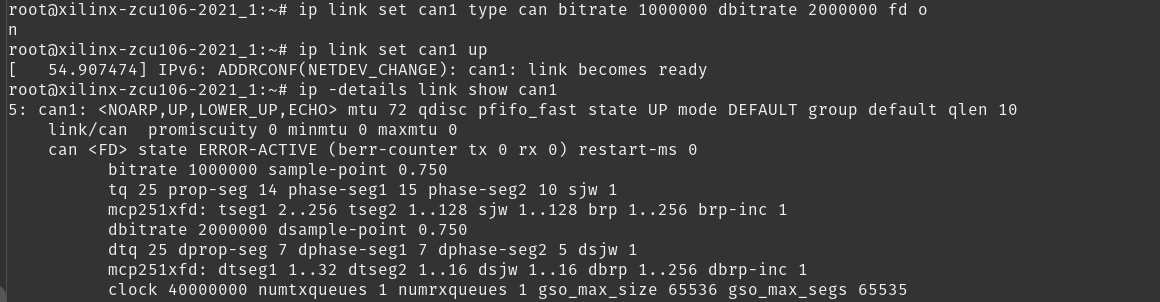
\includegraphics[width=1\textwidth]{./images/can_bitrate.jpg}
	\end{center}
	\vspace{-5pt}
	\caption[Inbetriebnahme des CAN-Mikrochips]{Inbetriebnahme des CAN-Mikrochips} % Eckige Klammer (optional): Caption-Text in Abbildungsverzeichnis
	\label{fig:can:inbetriebnahme}
	\vspace{-5pt}
\end{figure}

Um den CAN-Controller zu testen, wurde ein Host-Computer an einen CAN-Knoten angeschlossen. Der Computer sollte dann unter der Kontrolle des CAN-Controllers 64-Bit-Daten über den CAN-Bus an den Linux-Kernel senden. Dabei stehen die ersten 21 Bits für die Prüfsumme und die restlichen Bits für die gesendeten Daten. Diese Daten werden dann auf dem Linux-Terminal mit dem folgenden Linux Befehl angezeigt. 

\begin{lstlisting}[language=bash]
	$ candum can1
\end{lstlisting}

Folgenden Daten wurden an dem Linux Kernel gesendet. 

\begin{figure}[H]
	\begin{center}		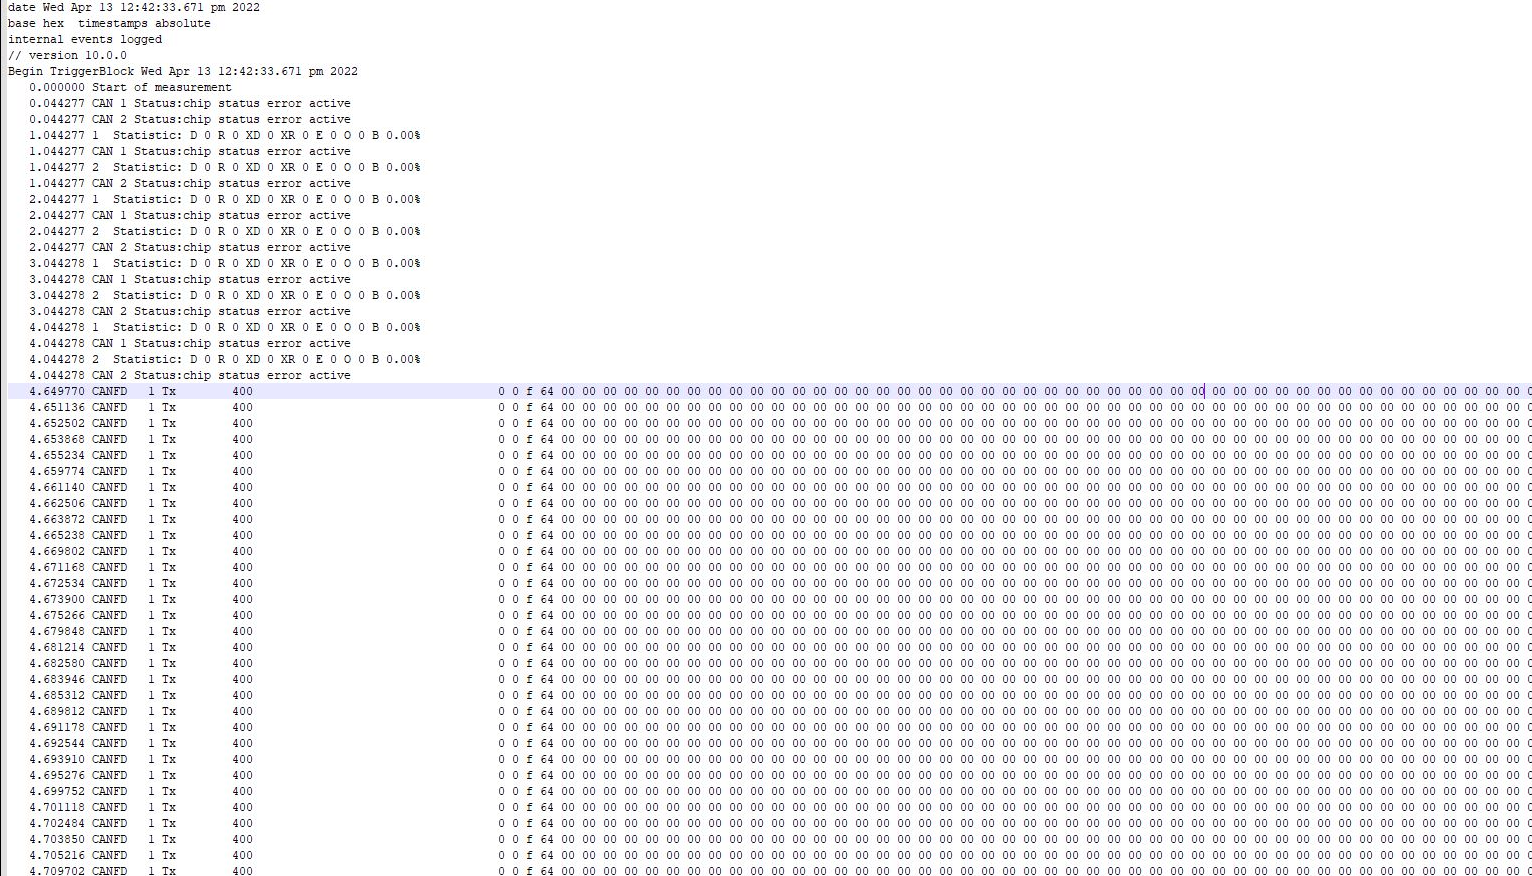
\includegraphics[width=1\textwidth]{./images/can_daten.jpg}
	\end{center}
	\vspace{-5pt}
	\caption[Gesendete CAN-Nachrichten]{Gesendete CAN-Nachrichten} % Eckige Klammer (optional): Caption-Text in Abbildungsverzeichnis
	\label{fig:gesendete:can:nachrichten}
	\vspace{-5pt}
\end{figure}

die folgenden CAN-Nachrichten wurden dann auf der Konsole empfangen. 

\begin{figure}[H]
	\begin{center}		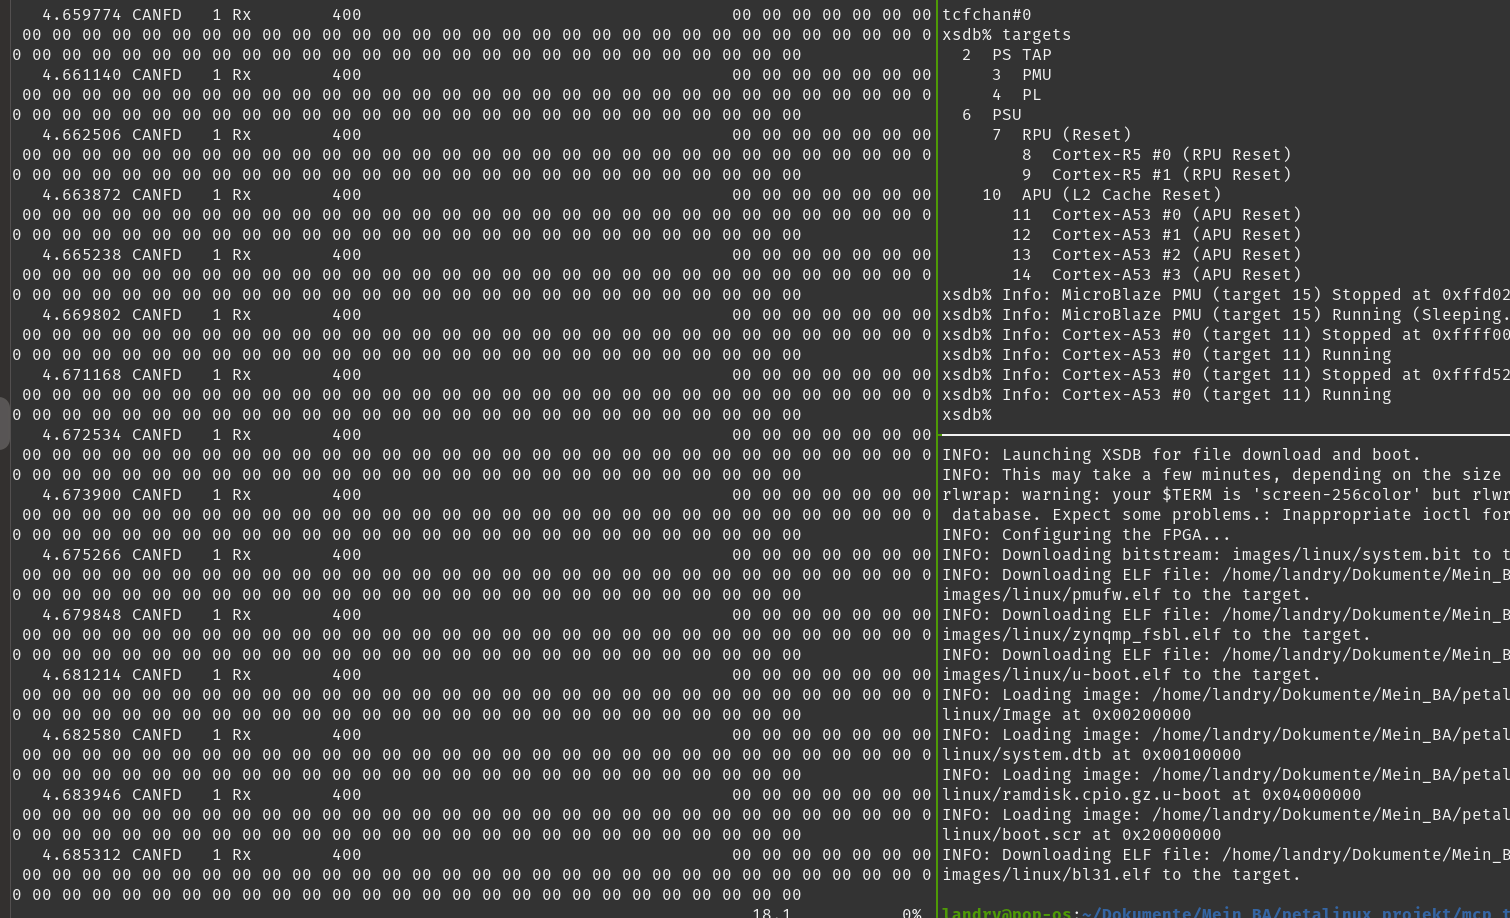
\includegraphics[width=1\textwidth]{./images/can_bootschaften.jpg}
	\end{center}
	\vspace{-5pt}
	\caption[Empfangene CAN-Nachrichten]{Empfangene CAN-Nachrichten} % Eckige Klammer (optional): Caption-Text in Abbildungsverzeichnis
	\label{fig:empfangene:can:nachrichten}
	\vspace{-5pt}
\end{figure}
Bis zu einer Buslast von etwa 70\% konnten Daten gesendet und empfangen werden, was ein hervorragendes Ergebnis ist. Im Normalbetrieb liegt die Buslast in der Regel bei etwa 25\%. 

In Abbildung ~\ref{fig:can:statistiken} ist die Statistik des Tests zu sehen
\begin{figure}[H]
	\begin{center}		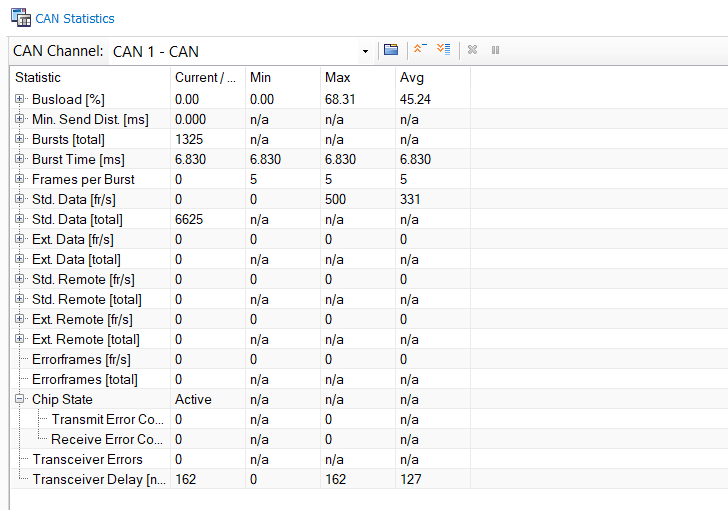
\includegraphics[width=1\textwidth]{./images/can_statistik.jpg}
	\end{center}
	\vspace{-5pt}
	\caption[Test Statistiken]{Test Statistiken} % Eckige Klammer (optional): Caption-Text in Abbildungsverzeichnis
	\label{fig:can:statistiken}
	\vspace{-5pt}
\end{figure}